\section{Zielsetzung}
Im Versuch soll die Wärmeleitfähigkeit von Aluminium, Messing und Edelstahl untersucht werden.

\section{Theorie}
Herrscht in einem Körper ein Temperaturungleichgewicht, so wird dieses mittels Wärmetransport
ausgeglichen. Dieser kann auf drei Arten stattfinden. Durch Konvektion, den Wärmetransport
makroskopischer Teilchen, durch Wärmestrahlung, den Wärmetransport mittels elektromagnetischer
Wellen und mittels Wärmeleitung, wobei die Wärme unter anderem über frei bewegliche Elektronen
und nicht durch makrsokopische Teilchenbewegung, weitergegeben wird.
Letzters wird im folgenden Versuch untersucht.
Dazu wird ein Stab der Länge $L$ mit Querschnittsfläche $A$, der Dichte $\rho$, der spezifischen
Wärme $c$ und der materialabhängigen Wärmeleitfähigkeit $\kappa$ betrachtet.
Die Wärmemenge $dQ$, die pro Zeit $dt$ transportiert wird, kann mittels folngenden
Zusammenhangs beschrieben werden:

\begin{equation*}
  \frac{dQ}{dt} = - \kappa A \frac{\partial T}{\partial x} .
\end{equation*}

Das Minuszeichen bedeutete, dass die Wärme vom kälteren, zum wärmeren Teil des Stabes fließt.
Die Wärmestromdichte beträgt folglich:

\begin{equation*}
  j_\symup{w} = - \kappa \frac{\partial T}{\partial x}
\end{equation*}

und mit Hilfe der Kontinuitätsgleichung folgt daraus die eindimensionale Wärmeleitungsgleichung:

\begin{equation*}
  \frac{\partial T}{\partial t} = \frac{\kappa}{\rho c} \frac{\partial^2 T}{\partial x^2}.
\end{equation*}

Die Größe $\sigma_\symup{T} = \frac{\kappa}{\rho c}$ beschreibt dabei, wie schnell sich
der Temperaturunterschied wieder ausgleicht und wird als Temperaturleitfähigkeit bezeichnet.

\noindent Die Temperaturwelle, die sich in einem Stab ausbreitet, welcher periodisch
erhitzt und abgekühlt wird, kann mit folgender Gleichung beschrieben werden:

\begin{equation*}
  T(x, t) = T_\symup{max} exp\left(- \sqrt{\frac{\omega \rho c}{2 \kappa}}x\right) cos \left(\omega t - \sqrt{\frac{\omega \rho c}{2 \kappa}} x\right),
\end{equation*}

die sich mit der Phasengeschwindigkeit
\begin{equation*}
  \nu = \sqrt{\frac{2 \omega \kappa}{\rho c}}
\end{equation*}

ausbreitet.
\FloatBarrier

Die Dämpfung wird aus dem Verhältnis zweier Amplituden$A_\symup{nah}$ und $A_\symup{fern}$
an zwei auseinanderliegenden Messstellen $x_\symup{nah}$ und $x_\symup{fern}$, zueinander bestimmt.
Wird außerdem

\begin{align*}
  \omega = \frac{2 \pi}{T^*} &&&& \Phi = \frac{2\pi \Delta t}{T^*}
\end{align*}

, mit $T^*$ für die Periodendauer der Phase $\Phi$ benutzt, so ergibt sich für die Wärmeleitfähigkeit:

\begin{equation}
  \label{eq:kappa}
  \kappa = \frac{\rho c (\Delta x)^2}{2 \Delta t \ln{(A_\symup{nah} / A_\symup{fern})}}.
\end{equation}

$\Delta x$ ist die Entfernung der beiden Messtellen und $\Delta t$ die Phasendifferenz
der Temperaturwelle an den beiden Messstellen.

\section{Durchführung}
Abbildung \ref{abb1} zeigt den Versuchsaufbau.
Die vier Stäbe sind zweimal Messing, und jeweils einmal Aluminium und Edelstahl.
Das Peltier Element dient dabei zum Erhitzen oder Abkühlen der Stäbe, je nach Schaltereinstellung.
Zu Beginn werden die Abstände $\Delta x$ zwischen den Thermoelementen gemessen und
das Netz- und Messgerät angeschlossen. Es ist darauf zu achten, dass die Stäbe während
jeder der Messungen isoliert sind, sodass der Wärmeaustausch mit der Umgebung möglichst gering
gehalten wird.

\begin{figure}
  \centering
  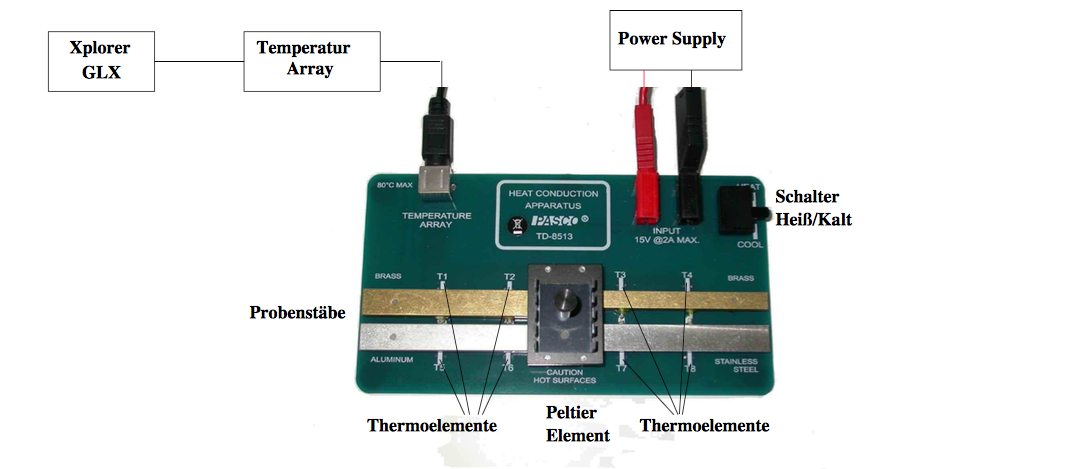
\includegraphics[scale=0.4]{Aufbau.PNG}
  \caption{Versuchsaufbau \cite{Quelle}}
  \label{abb1}
\end{figure}

\subsection{Statische Methode}
Zur Durchführung der statischen Methode wird die Spannung des Netzgeräts auf $\SI{8}{\volt}$ und die
Abtastrate des Messgeräts auf $\SI{5}{\per \second}$ eingestellt. Der Schalter am Peltier Element wird
nun auf "Heat" gestellt, sodass sich die Stäbe erwärmen. Hat der Edelstahlstab eine Temperatur
von $\SI{45}{\degree}$ erreicht, so werden anschließend alle Stäbe auf $\SI{30}{\degree}$ abgekühlt
und die Messwerte exportiert.

\subsection{Dynamische Mehode}
Bei der dynamischen Methode, wird eine Spannung am Netzgerät von $\SI{11}{\volt}$ und
eine Abtastrate von $\SI{2}{\second}$ benötigt. Dann werden alle vier Stäbe alternierend
für $\SI{40}{\second}$ erhitzt und abgekühlt. Dies wird für 12 Perioden durchgeführt.
Abermals werden die Messwerte exportiert und die Stäbe auf $\SI{30}{\degree}$
abgekühlt. Anschließend folgt analog der zweite Durchgang, in dem die Stäbe jeweils für
$\SI{100}{\second}$ alternieren erhitzt und abgekühlt werden, die Messwerte gespeichert und exportiert werden.


\section{Auswertung}

\subsection{Statische Methode}
Bei der statischen Methode werden die Stäbe ohne Unterbrechung erhitzt und die Temperaturen in der
Nähe und $\SI{4}{\centi\meter}$ von der beheitzten Stelle entfernt gemessen.
Die gemessenen Temperaturen werden im Diagramm \ref{Abb:1} dargestellt.

\begin{figure}
  \centering
  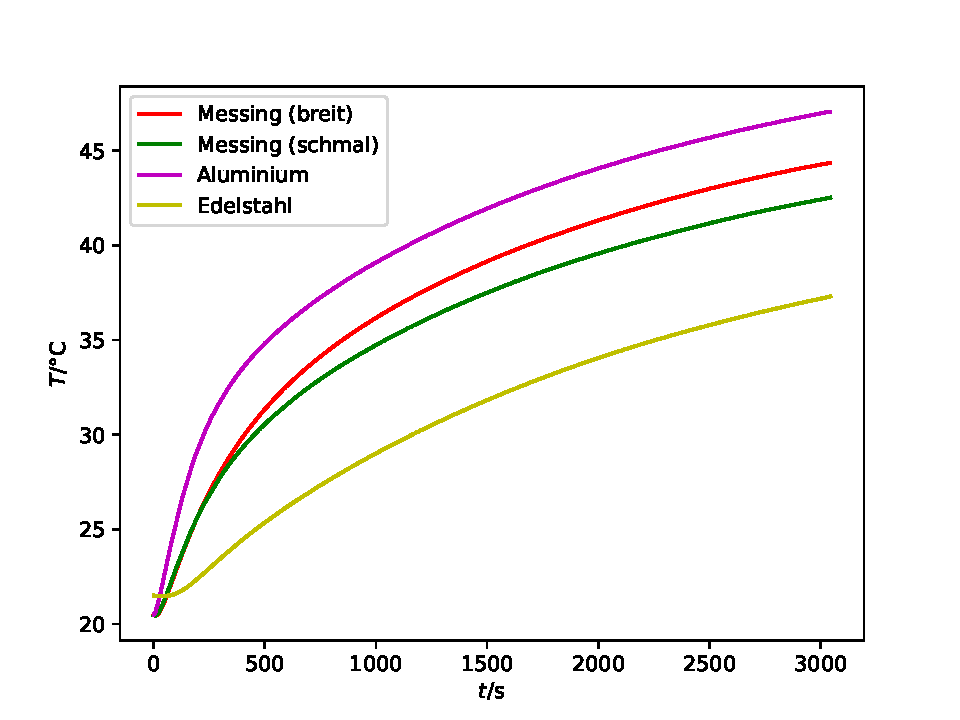
\includegraphics[scale = 0.7]{plotA.pdf}
  \caption{Messungen der Temperatur bei der statischen Methode.}
  \label{Abb:1}
\end{figure}


Nach $\SI{700}{\second}$ lassen sich folgende Temperaturen aus der Wertetabelle ablesen:
\begin{align*}
  T_\symup{Messing(breit)} &= \SI{33.64}{\celsius} \\
  T_\symup{Messing(schmal)} &= \SI{32.51}{\celsius} \\
  T_\symup{Aluminium} &= \SI{36.81}{\celsius} \\
  T_\symup{Edelstahl} &= \SI{26.95}{\celsius} \\
\end{align*}
Zu erkennen ist, dass Aluminium der beste Wärmeleiter der 4 Probestäbe darstellt und  Edelstahl der schlechteste.
Aus den Verläufen der Messingstäbe lässt sich schließen, dass schmale Stäbe die Wärme besser leiten, als dickere.
Dennoch ist zu erkennen, dass die Verläufe der Messingstäbe sich am Anfang kaum unterscheiden, erst ab ca.
$\SI{250}{\second}$ laufen beiden Graphen auseinander.
Alle Graphen steigen zunächst stark an und ab ca. $\SI{1500}{\second}$ lässt sich fast ein geradlinieger Verlauf erkennen.


Zur Berechnung des Wärmestroms $ \frac{\Delta Q}{\Delta t} $ zu 5 verschienden Messzeiten (\SI{500}{\second}, \SI{1000}{\second},
\SI{1500}{\second}, \SI{2000}{\second}, \SI{2500}{\second}) die Messwerte abgelesen und in die Formel

\begin{equation}
  \frac{\Delta Q}{\Delta t} = - \kappa A \frac{T_1-T_2}{dx}
\end{equation}

eingesetzt. Dafür werden folgende Literaturwerte für \kappa

\begin{align*}
  \kappa_\symup{Messing} &= \SI{120}{\watt\per\meter\per\kelvin} \\
  \kappa_\symup{Aluminium} &= \SI{236}{\watt\per\meter\per\kelvin} \\
  \kappa_\symup{Edelstahl} &= \SI{20}{\watt\per\meter\per\kelvin} \\
\end{align*}

und die gegebenen Werte für die Querschnittsfläche $A$ eingesetzt

\begin{align*}
  A_\symup{Messing(breit)} &= \SI{0.48e-4}{\meter^2} \\
  A_\symup{Messing(schmal)} &= \SI{0.24e-4}{\meter^2} \\
  A_\symup{Aluminium} &= \SI{0.48e-4}{\meter^2} \\
  A_\symup{Edelstahl} &= \SI{0.48e-4}{\meter^2} \, , \\
\end{align*}

wobei $dx = \SI{3}{\centi\meter}$ den Messabstand der Temperaturen beschreibt. Die Messwerte und Ergebnisse sind
in Tabelle \ref{tab:10} aufgelistet.

 \begin{table}
   \centering
   \caption{Wärmestrom}
   \label{tab:10}
   \begin{tabular}{c c | c}
     \toprule
     $T_\symup{nah}$ / \si{\celsius} & $T_\symup{fern}$ / \si{\celsius} & $\frac{\Delta Q}{\Delta t}$ / \si{\watt} \\
     \midrule
     Messing (breit) & & \\
     \midrule
     33.53 & 31.33 & -0.422 \\
     37.96 & 36.13 & -0.352 \\
     40.89 & 39.15 & -0.334 \\
     43.05 & 41.31 & -0.334 \\
     44.72 & 42.98 & -0.334 \\
     \midrule
     Messing (schmal) & & \\
     \midrule
     33.45 & 30.55 & -0.279 \\
     37.45 & 34.73 & -0.261 \\
     40.25 & 37.49 & -0.265 \\
     42.35 & 39.56 & -0.268 \\
     43.97 & 41.16 & -0.269 \\
     \midrule
     Aluminium & & \\
     \midrule
     36.20 & 34.82 & -0.525 \\
     40.30 & 39.09 & -0.457 \\
     43.14 & 41.93 & -0.457 \\
     45.28 & 44.06 & -0.461 \\
     46.90 & 45.68 & -0.461 \\
     \midrule
     Edelstahl & & \\
     \midrule
     32.99 & 25.35 & -0.244 \\
     36.79 & 29.00 & -0.249 \\
     39.64 & 31.82 & -0.251 \\
     41.84 & 34.04 & -0.249 \\
     43.54 & 35.79 & -0.248 \\
     \bottomrule
   \end{tabular}
 \end{table}

In Abbildung \ref{Abb:2} sind die Temperaturdifferenzen der nahen und fernen Temperaturmessung für Messing (breit)
und Edelstahl dargestellt. Der Graph der Temperaturdiffernez von Edelstahl nähert sich nach einiger Zeit ca. an den Wert
\SI{7.8}{\celsius} wie eine Exponentialfunktion an.
Bei Messing hingegen steigt der Wert zunächst auf ein Maximum bei ca. \SI{3}{\celsius} an, um darauf folgend sich einem Wert
von \SI{2}{\celsius} anzunähern.
Zusammenfassend ist zu erkennen, dass Aluminium der beste Wärmeleiter ist und Edelstahl der schlechteste von den
Probestäben.

\begin{figure}
  \centering
  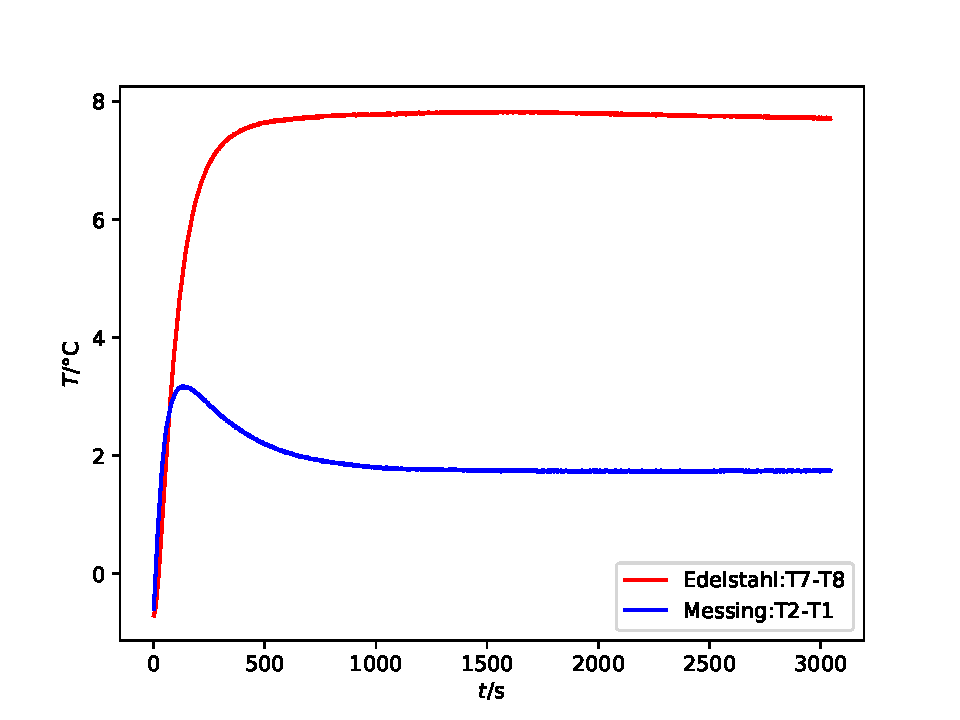
\includegraphics[scale = 0.7]{plotB.pdf}
  \caption{Temperaturdifferenzen für Messing(breit) und Edelstahl.}
  \label{Abb:2}
\end{figure}


\subsection{Dynamische Methode}

Bei der dynamischen Methode werden die Stäbe in Intervallen erhitzt und direkt wieder abgekühlt.

\subsubsection{Wärmeleitkoeffizient Messing}

Zunächst wird eine Messung mit einer Periodendauer von $ T = \SI{80}{\second}$ durchgeführt bzw. mit einer Frequenz von $ f = \SI{0.0125}{\per\second}$ ,
und die Werte für Messing in Abbildung \ref{Abb:3} und für Aluminium in Abbildung \ref{Abb:4} dargestellt.
Die Amplituden $A_\symup{nah}$, $A_\symup{fern}$ und die Phasendifferenz $\Delta t$ in Tabelle \ref{tab:1}
werden der Wertetabelle für die Graphik in Abbildung \ref{Abb:3} entnommen.

\begin{figure}
  \centering
  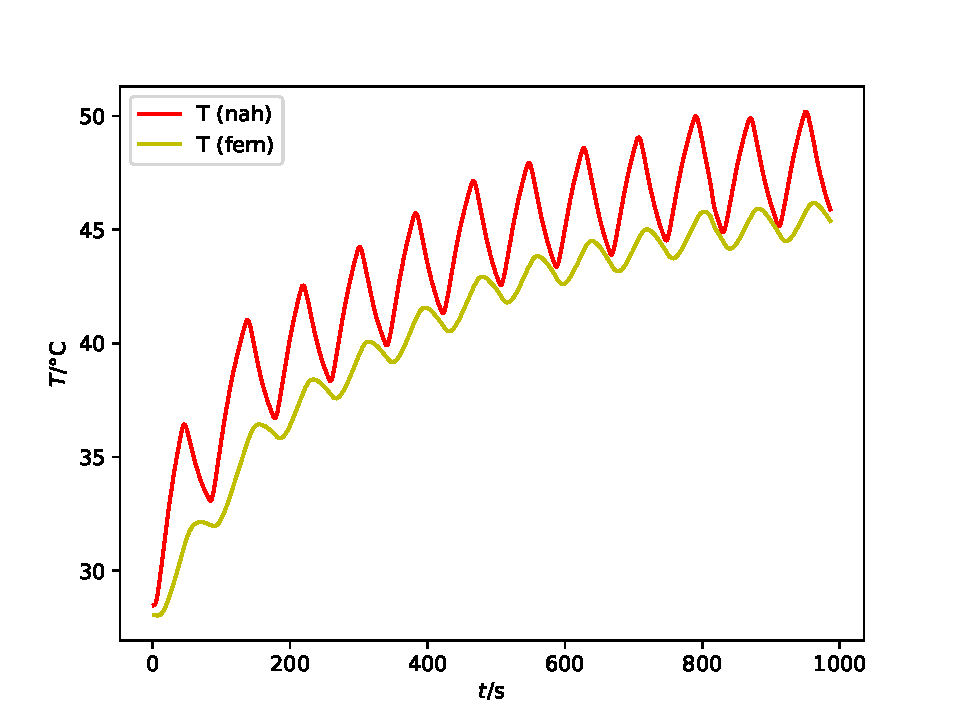
\includegraphics[scale = 0.7]{plotCMessing.pdf}
  \caption{Dynamische Methode, Messing.}
  \label{Abb:3}
\end{figure}


\begin{table}
  \centering
  \caption{Messung der Amplituden und der Phasendifferenz, Messing.}
  \label{tab:1}
  \begin{tabular}{c c c | c}
    \toprule
    $A_\symup{fern}$ / \si{\celsius} & $A_\symup{nah}$ / \si{\celsius} & $\Delta t$ / \si{\second} & $\kappa$ / \si{\watt\per\meter\per\kelvin}\\
    \midrule
    2.05 & 3.98 & 24 & 92.53 \\
    2.05 & 3.99 & 16 & 138.79 \\
    1.30 & 2.92 & 14 & 129.67 \\
    1.25 & 2.95 & 12 & 143.54 \\
    1.20 & 2.90 & 14 & 119.49 \\
    1.21 & 2.91 & 14 & 119.59 \\
    1.02 & s.69 & 12 & 126.85 \\
    0.95 & 2.62 & 12 & 120.63 \\
    0.93 & 2.56 & 12 & 121.07 \\
    1.03 & 2.73 & 12 & 126.19 \\
    0.88 & 2.52 & 12 & 116.29 \\
    0.84 & 2.52 & 10 & 134.60 \\
    \bottomrule
  \end{tabular}
\end{table}

Aus den Werten aus Tabelle \ref{tab:1} und den Literaturwerten für die Dichte $\rho$ und der spezifischen
Wärmekapazität $c$

\begin{align*}
  \rho_\symup{Messing} &= \SI{8520}{\kilogram\per\meter^3}  \\
  c_\symup{Messing} &= \SI{385}{\joule\per\kilogram\per\kelvin}
\end{align*}

lässt sich der Wärmeleitkoeffizient $\kappa$ mit Hilfe der Formel \eqref{eq:kappa}
für Messing berechnen. Aus den einzelnen Werten für $\kappa_\symup{Messing}$ lässt sich der Mittelwert und der Fehler mittels
 Standardabweichung  berechnen.

\begin{equation}
  \overline{\kappa}_\symup{Messing} = \SI{124(4)}{\watt\per\meter\per\kelvin}
\end{equation}

Zur Berechnung der Wellenlänge wird die Formel

\begin{equation}
  \label{Wellenlänge}
  \lambda = \sqrt{\frac{4 \pi \, \overline{\kappa}\, T }{\rho c}}
\end{equation}

verwendet, hierbei ist $\overline{\kappa}$ der vorher berechnete materialspezifische Wärmeleitkoeffizient, $T$ die Periodendauer, $\rho$ die
Dichte des Mediums und $c$ die spezifische Wärmekapazität.
Durch einsetzten der Werte für Messing erhält man folgenden Wellenlänge

\begin{equation*}
  \lambda_\symup{Messing} = \SI{26.0(4)}{\centi\meter}
\end{equation*}

\subsubsection{Wärmeleitkoeffizient Aluminium}

\begin{figure}
  \centering
  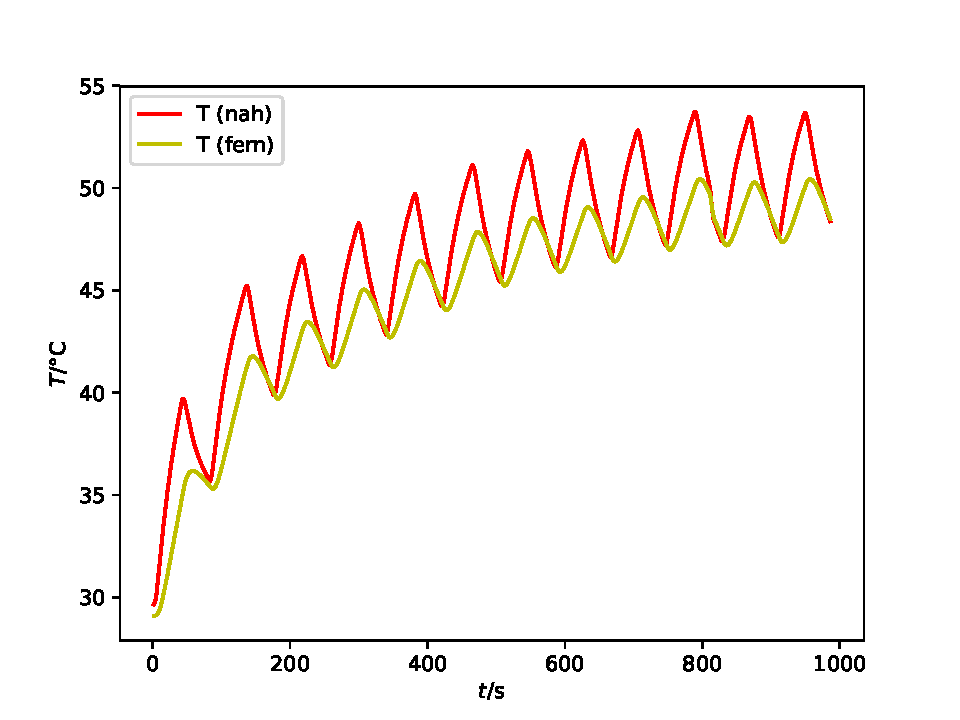
\includegraphics[scale = 0.7]{plotCAluminium.pdf}
  \caption{Dynamische Methode, Aluminium.}
  \label{Abb:4}
\end{figure}

Die Berechnung für den Wärmeleitkoeffizienten $\kappa_\symup{Aluminium}$ für Aluminium läuft analog zu
der für Messing. Die Frequenz der Messreihe bleibt bei $f = \SI{0.0125}{\per\second}$.

\begin{align*}
  \rho_\symup{Aluminium} &= \SI{2800}{\kilogram\per\meter^3}  \\
  c_\symup{Aluminium} &= \SI{830}{\joule\per\kilogram\per\kelvin}
\end{align*}

Zunächst werden die Amplituden $A_\symup{nah}$, $A_\symup{fern}$ und die Phasendifferenz $\Delta t$ der
Wertetabelle entnommen und in die Gleichung \eqref{eq:kappa} eingesetzt. Die aus der Wertetabelle entnommenen Werte und
die berechneten Werte für $\kappa$ sind in Tabelle \ref{tab:2} aufgelistet.

\begin{table}
  \centering
  \caption{Messung der Amplituden und der Phasendifferenz, Aluminium.}
  \label{tab:2}
  \begin{tabular}{c c c | c}
    \toprule
    $A_\symup{fern}$ / \si{\celsius} & $A_\symup{nah}$ / \si{\celsius} & $\Delta t$ / \si{\second} & $\kappa$ / \si{\watt\per\meter\per\kelvin}\\
    \midrule
    3.52 &  5.03 & 16 & 185.10 \\
    3.25 &  4.75 & 10 & 274.47 \\
    1.88 &  3.39 & 10 & 176.59 \\
    1.90 &  3.47 & 8  & 217.56 \\
    1.88 &  3.43 & 8  & 215.50 \\
    1.92 &  3.46 & 8  & 221.53 \\
    1.65 &  3.19 & 8  & 198.29 \\
    1.59 &  3.09 & 8  & 195.82 \\
    1.33 &  3.09 & 8  & 154.38 \\
    1.73 &  3.26 & 6  & 275.09 \\
    1.52 &  3.04 & 8  & 192.69 \\
    1.55 &  3.05 & 8  & 192.21 \\
    \bottomrule
  \end{tabular}
\end{table}

Durch Bildung des Mittelwertes und des Fehlers mittels Standardabweichung folgt für den Wärmeleitkoeffizienten
von Aluminium $\kappa_\symup{Aluminium}$

\begin{equation*}
  \overline{\kappa}_\symup{Aluminium} = \SI{208(10)}{\watt\per\meter\per\kelvin}
\end{equation*}

Auch hier wird die Wellenlänge mit Hilfe der Formel \ref{Wellenlänge} berechnet, durch einsetzen der Werte folgt

\begin{equation*}
  \lambda_\symup{Aluminium} = \SI{30.0(8)}{\centi\meter}
\end{equation*}

\subsubsection{Wärmeleitkoeffizient Edelstahl}

Die Berechnung des Wärmeleitkoeffizienten $\kappa$ von Edelstahl läuft analog zu der von Messing und Aluminium. Die Messung wird hierbei mit
einer Periodendauer von \SI{200}{\second}, bzw. einer Freuquenz von $f = \SI{0.005}{\per\second}$ durchgeführt.
Hierzu werden aus den Messwerten die Werte für die Amplituden $ A_\symup{nah}$, $A_\symup{fern}$ und die
Phasenverschiebung $\Delta t$ entnommen. Die Literaturwerte für die Dichte $\rho$ und die spezifische
Wärmekapazität $c$ sind durch

\begin{align*}
  \rho_\symup{Edelstahl} &= \SI{8000}{\kilogram\per\meter^3}  \\
  c_\symup{Edelstahl} &= \SI{400}{\joule\per\kilogram\per\kelvin}
\end{align*}

gegeben. Die gemessenen und berechneten Werte sind in Tabelle \ref{ŧab:3} aufgelistet.


\begin{table}
  \centering
  \caption{Messung der Amplituden und der Phasendifferenz, Edelstahl.}
  \label{tab:3}
  \begin{tabular}{c c c | c}
    \toprule
    $A_\symup{nah}$ / \si{\celsius} & $A_\symup{fern}$ / \si{\celsius} & $\Delta t$ / \si{\second} & $\kappa$ / \si{\watt\per\meter\per\kelvin}\\
    \midrule
    5.25  & 1.72 & 92 & 14.00 \\
    5.23  & 1.52 & 90 & 12.91 \\
    5.04  & 1.34 & 84 & 12.94 \\
    4.85  & 1.09 & 70 & 13.79 \\
    4.71  & 1.01 & 66 & 14.12 \\
    4.59  & 0.86 & 58 & 14.78 \\
    4.52  & 0.79 & 52 & 15.94 \\
    4.46  & 0.69 & 48 & 16.02 \\
    4.30  & 0.60 & 46 & 15.89 \\
    4.42  & 0.63 & 50 & 14.73 \\
    4.41  & 0.61 & 52 & 13.95 \\
    4.38  & 0.57 & 50 & 14.07 \\
    \bottomrule
  \end{tabular}
\end{table}

Durch Bildung des Mittelwertes und der Standardabweichung konnte folgeneder Wert für die Wärmeleitfähigkeit
von Edelstahl ermittelt werden

\begin{equation*}
  \overline{\kappa}_\symup{Edelstahl} = \SI{14.4(3)}{\watt\per\meter\per\kelvin} \, .
\end{equation*}

Auch hier wird die Wellenlänge mit Hilfe der Formel \ref{Wellenlänge} berechnet, durch einsetzen der Werte folgt

\begin{equation*}
  \lambda_\symup{Edelstahl} = \SI{10.6(1)}{\centi\meter}
\end{equation*}

\begin{figure}
  \centering
  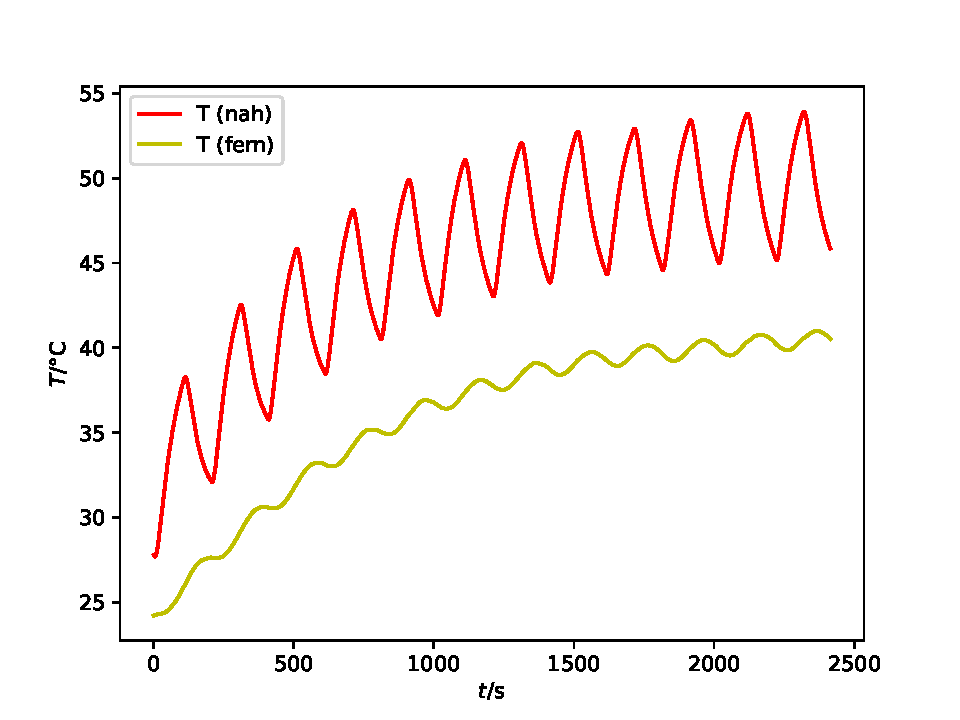
\includegraphics[scale=0.7]{plotCEdelstahl.pdf}
  \caption{Dynamische Methode für Edelstahl.}
  \label{Abb:5}
\end{figure}

\section{Diskussion}

In Tabelle \ref{tab:4} sind die berechneten Wärmekapazitäten den Literaturwerten gegenübergestellt.
Zu erkennen sind Abweichungen von bis zu \SI{28}{\percent}. Mögliche systematische Fehler können durch die
nicht vollständige Wärmeisolation der Stäbe auftreten, da somit ein Wärmeaustausch mit der Umgebung stattfindet.
Ein weiterer Fehler ist die Abtastrate des Geräts, da diese zwar vorher eingestellt wurde, aber die Einstellug so nicht
stimmen kann, da wir sonst viel zu lange gemessen hätten.
\begin{table}
  \centering
  \caption{Vergleich der Wärmekapazitäten mit den Literaturwerten.}
  \label{tab:4}
  \begin{tabular}{c | c c c}
    \toprule
    & $\kappa_\symup{berechnet}$ / \si{\watt\per\meter\per\kelvin} &
    $\kappa_\symup{Literaturwert}$ / \si{\watt\per\meter\per\kelvin} &
    $\Delta \kappa$ / \si{\percent} \\
    \midrule
    Messing & \num{124(4)} &  120 & 3.3 \\
    Aluminium & \num{208(10)} & 236 & 11.9\\
    Edelstahl & \num{14.4(3)} & 20 & 28.0 \\
    \bottomrule
  \end{tabular}
\end{table}

\nocite{*}
\printbibliography
